\title{VerifiQuant: Governance-by-Execution for Financial LLM Workflows}

\author{Anonymous Author(s)}
\affiliation{\institution{Anonymous Institution}\country{}}

\begin{abstract}
Large language models embedded in financial workflows fail most dangerously by emitting confident, well-formatted, wrong numbers with no signal distinguishing them from correct ones.
We argue the deployment problem is \emph{governability}: a system must know when a question is out of scope, incomplete, boundary-violating, or ambiguous, and intercept, clarify, or refuse in a structured, auditable way.
We present \textbf{VerifiQuant}, which compiles these query-qualification checks into runtime controls.
Each formula family becomes a \emph{Financial Inference Contract} (applicability conditions, typed inputs, deterministic computation, numerical invariants, declared semantic ambiguities), and every query passes an executable M/N/F/E/I/C diagnostic funnel whose exits are attributable outcomes; the LLM only maps into contracts, while financial computation stays deterministic.
A matched retrieval-plus-execution baseline (R-PAL) that shares our backbone, top-4 retrieval, and deterministic execution \emph{ties} VerifiQuant on clean, well-posed questions---clean scalar accuracy is not our claim.
The systems separate on contract-derived inputs with no valid numeric answer, where executed gates cut false numeric acceptance to \govVQfnar{} versus \govPlainFnar{} (plain R-PAL) and \govPromptFnar{} (the same R-PAL prompted with our full governance taxonomy).
We then characterize the boundary and its cost: abstention tracks contract coverage, out-of-library coverage is traded for a verified/unverified boundary, and residual errors localize to selection, binding, and specification frontiers.
\end{abstract}

\begin{CCSXML}
<ccs2012>
<concept><concept_id>10010405.10003550</concept_id><concept_desc>Applied computing~Economics</concept_desc><concept_significance>500</concept_significance></concept>
<concept><concept_id>10010147.10010178</concept_id><concept_desc>Computing methodologies~Artificial intelligence</concept_desc><concept_significance>500</concept_significance></concept>
</ccs2012>
\end{CCSXML}
\ccsdesc[500]{Applied computing~Economics}
\ccsdesc[500]{Computing methodologies~Artificial intelligence}
\keywords{financial reasoning, LLM governance, selective prediction, neuro-symbolic systems, auditability}

\maketitle

\section{Introduction}
Financial institutions are deploying large language models (LLMs) in workflows that end in numbers: valuation memos, portfolio analytics, client calculators, regulatory reports.
Benchmark accuracy has climbed, and it is tempting to treat the remaining gap as one more model generation away from solved.
We argue that framing misses what blocks deployment: a financial workflow fails in production less because it computes the wrong number than because \emph{nobody can govern when it should output a number at all}.
A deployable system must also know when \emph{not} to answer---when a question is out of scope, missing required inputs, boundary-violating, or ambiguous in a way that changes the computation.

Deterministic execution addresses the arithmetic but not these qualification failures.
A syntactically perfect program can compute the wrong financial semantics, force-fit a formula the library does not contain, or answer a question whose inputs are absent.
In our trap study a strong execution baseline responds to a ``Heston stochastic-volatility'' pricing request by computing an unrelated manufacturing ratio from the surrounding context: the code runs, and the number is confidently wrong.

This distinction has a sharp empirical consequence.
The fairest baseline we can build---R-PAL, which writes and deterministically executes a program over the \emph{same} top-4 retrieved contracts VerifiQuant uses---already \emph{matches} VerifiQuant on clean, well-posed questions (\S\ref{sec:v2res}).
The two systems separate most clearly on inputs that do not support a legitimate numeric answer, where executed governance intercepts what execution alone force-fits.
Clean-set accuracy is therefore not our contribution; \emph{governed behavior on malformed inputs} is.

The controls we execute are motivated by recurring model-risk, auditability, and human-oversight requirements for high-stakes AI \cite{fed2011sr117,euaiact2024,finra2020ai}: declare scope boundaries, validate inputs, disclose ambiguity, log reproducibly, and route to human checkpoints where the system cannot resolve a question autonomously.
We do not claim regulatory compliance; we borrow these requirements only to define design targets.

\textbf{Contributions.}
\emph{First}, we introduce governance by execution for formula-grounded financial reasoning.
Financial Inference Contracts combine applicability conditions, typed inputs, deterministic computation, numerical invariants, and declared semantic ambiguities; an executable diagnostic funnel turns refusal, clarification, and computation into structured, attributable outcomes.
\emph{Second}, we isolate governance from retrieval and execution using a matched R-PAL baseline that receives the same top-4 contracts and executes generated programs deterministically.
R-PAL matches VerifiQuant on clean, well-posed questions, delimiting our claim; the systems separate on contract-derived malformed inputs with no valid numeric answer, where executed gates reduce false numeric acceptance beyond both plain and taxonomy-prompted R-PAL.
\emph{Third}, we characterize the boundary and cost of this guarantee through library-coverage sweeps and failure attribution: VerifiQuant trades out-of-library answer coverage for a contract-grounded verified/unverified boundary, and clarification-assisted results are reported only as an intent-aware upper-bound analysis.

\emph{Scope.} Our evaluated territory is the formula-grounded numerical core: single questions whose answer is a deterministic computation over inputs extractable from the given context.
Multi-document extraction, data freshness, jurisdictional policy, and non-numerical judgment are out of scope.

\section{Problem Formulation and Related Work}\label{sec:v2problem}
We frame the deployment question directly: \emph{given a financial question and context, when is emitting a numeric answer legitimate?}
Each response falls into one of three outcomes: a \textbf{correct} numeric answer, a \textbf{silent wrong} (a confident, unflagged, incorrect number), or a \textbf{structured abstention/clarification} that names why no answer was emitted.
We measure \emph{coverage} (fraction answered), \emph{selective accuracy} (correct among answered), \emph{silent-wrong rate} (SWR, silent wrongs over all items), and, on adversarial inputs, \emph{false numeric acceptance rate} (FNAR).
Silent-wrong rate is the key deployment-risk metric; informal prose refusals are counted as abstention, not silent wrong, for every system.

A note on FNAR is essential.
In the trap set, no legitimate \emph{unqualified single} numeric answer exists: a required field is missing, a declared boundary is violated, a material convention remains unresolved, or the ask is outside the evaluated task scope.
Any un-intercepted number is therefore a false numeric acceptance by construction, not an ordinary accuracy error: the correct behavior is interception, clarification, or slot-filling, and emitting a confident single number is unsafe.

\emph{Program-aided reasoning.}
PAL and Program-of-Thoughts \cite{gao2023pal,chen2023pot} delegate arithmetic to an interpreter, addressing computation errors.
They do not qualify the query: a perfectly executing program can still encode the wrong formula, binding, or convention, with no signal that it did.

\emph{Neuro-symbolic methods.}
Logic-LM, LINC, and SAT-LM \cite{pan2023logiclm,olausson2023linc,ye2023satlm} obtain guarantees by translating language into solver input, but the translation step is the dominant error source, and specification synthesis is undecidable in general \cite{zhou2026formaljudge}.
VerifiQuant moves formalization offline: contracts are built and validated at build time, so runtime only selects and binds within a pre-verified space.

\emph{Selective prediction.}
Answer-or-abstain methods \cite{elyaniv2010foundations,geifman2017selective} typically threshold a confidence score.
VerifiQuant instead abstains on \emph{contract-declared checks}---scope, schema, boundary, ambiguity---rather than a calibrated probability, yielding an exit that names which check failed.

\emph{Financial LLM governance.}
Model-risk, auditability, and oversight requirements \cite{fed2011sr117,euaiact2024,finra2020ai} motivate our controls but define targets, not a compliance claim.
Multi-agent financial systems \cite{kundu2025multiagent} add natural-language consensus in which failures propagate silently across agents \cite{cemri2025mas}; we treat such a system only as a supporting pilot comparison and defer its full analysis.

\section{VerifiQuant}\label{sec:v2method}
\subsection{Financial Inference Contract}
An FIC packages one formula family into four essentials keyed by \texttt{fic\_id}: (i) \emph{applicability and non-applicability} conditions plus retrieval metadata that decide whether the contract applies; (ii) \emph{typed inputs}; (iii) \emph{deterministic compute} code in plain Python; and (iv) \emph{numerical invariants and declared semantic ambiguities} (period timing, percent-versus-decimal, unit basis), each ambiguity carrying resolution options and a hard/soft level.
The LLM's role is \emph{mapping into contracts}---selecting, binding, and flagging---never performing the financial computation.
Contracts are governed at build time: compute code passes execution smoke tests, invariant expressions are lint-gated against the exact runtime evaluation namespace, and a pre-declared output-type policy is enforced by audit.
The 250-card library used here is generated fully automatically (three staged LLM calls per family plus deterministic normalization) and never reads any per-question worked solution or gold answer.

\subsection{Executable diagnostic funnel}
\begin{figure*}[t]
\centering
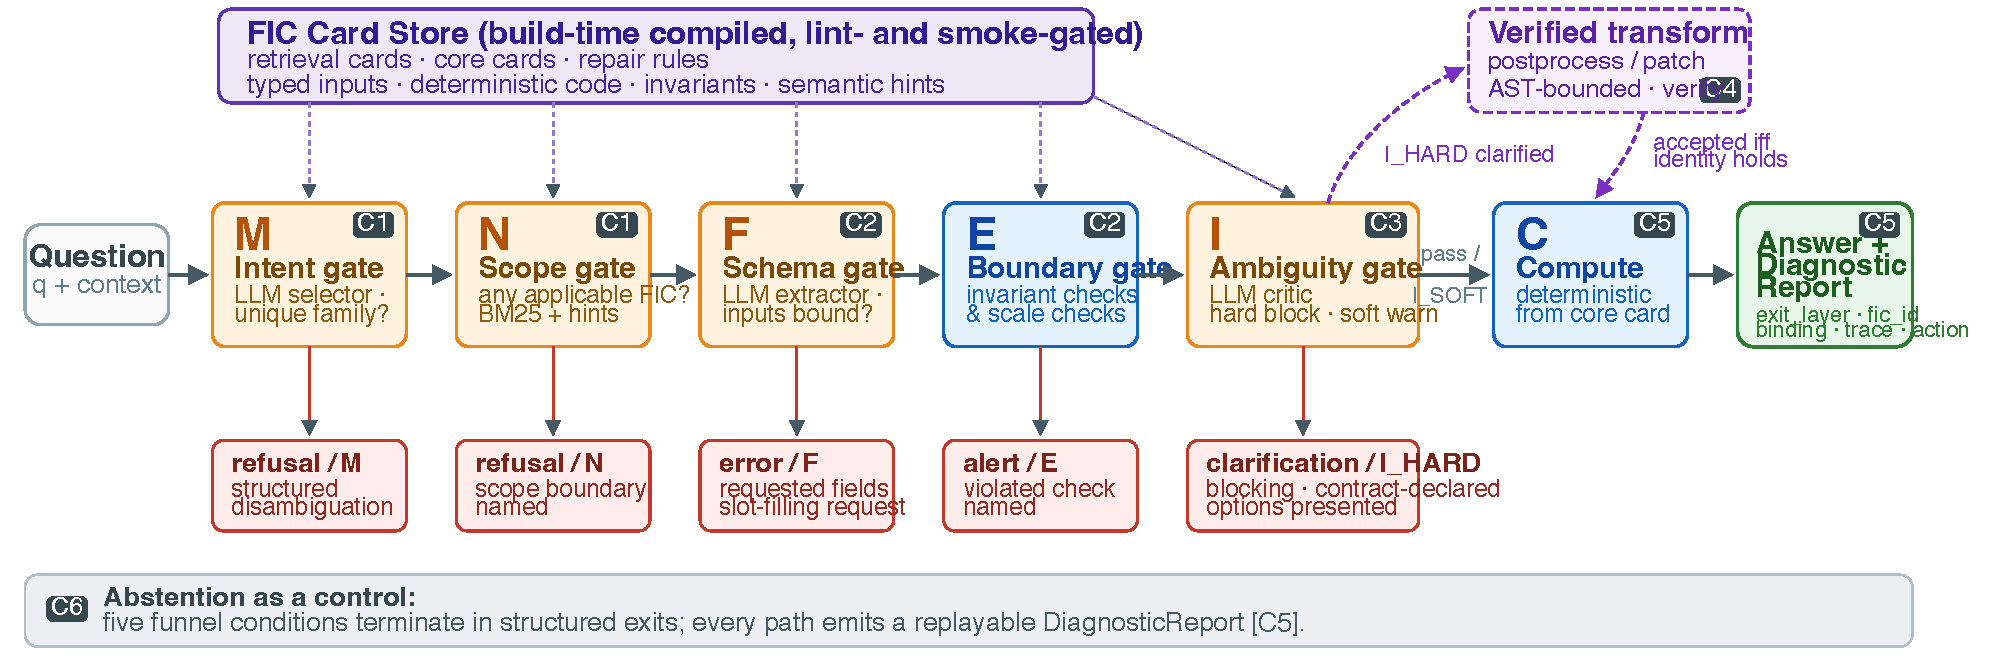
\includegraphics[width=\linewidth]{figures/fig1_pipeline_big.pdf}
\caption{The VerifiQuant pipeline.
LLM components (orange) only map into contracts; all financially consequential computation is deterministic (blue).
Five funnel conditions terminate in structured exits (red); repairs go through verified atomic transforms (purple).
Badges C1--C6 mark the governance controls (scope declaration, input validation, ambiguity disclosure, cross-verified repair, audit-replayable trace, abstention).}
\label{fig:v2pipeline}
\end{figure*}
Given a question and context, gates fire in order and each produces a \emph{DiagnosticReport} (Figure~\ref{fig:v2pipeline}).
\textbf{M/N} ask whether exactly one applicable contract exists; the exit is a structured disambiguation request or a scope-boundary refusal.
\textbf{F/E} ask whether the inputs are complete and satisfy the contract's deterministic checks; the exit is a slot-filling request or a boundary alert naming the violated check.
\textbf{I} asks whether an unresolved declared ambiguity would change the computation (blocking I\textsubscript{HARD}) or only its interpretation (warning I\textsubscript{SOFT}).
\textbf{C} performs deterministic execution with an audit log.
Abstention is not a fallback: five funnel conditions can terminate in a structured non-answer exit, while I\textsubscript{SOFT} proceeds with a warning and C computes.

Auditability is scoped precisely.
Deterministic execution and invariant evaluation replay exactly from the stored binding, and LLM-mediated selection and binding decisions are logged so a historical decision can be re-executed as recorded; a fresh rerun from raw text is \emph{not} guaranteed to take the identical path.
Across four independent reruns of a canonical subset, outcomes remain stable while recovery paths vary.

\subsection{Bounded repair}
When an I\textsubscript{HARD} clarification changes the required computation, free-form regeneration would reopen the door the funnel just closed.
Repairs are therefore restricted to AST-bounded transforms whose numerical effect must match a contract-declared algebraic relation at the point of use, checked on multiple sampled inputs before acceptance.
This is bounded numerical validation, not formal equivalence: single-sided errors are caught, while a wrong invariant paired with a compensating patch would pass.
A mutation audit over the synthesizable transforms in the 250-card library rejects \textbf{97.7\%} of non-equivalent wrong patches (structural attacks at 100\%); the mutation-class breakdown is deferred.

\section{Experimental Design}\label{sec:v2design}
\subsection{Clean in-library evaluation}
We evaluate on 250 FinanceReasoning \cite{tang2025financereasoning} questions (180 medium, 70 hard), drawn from the function-linked subset in which each question carries a formula-level reference implementation.
The contract library is built from those reference functions; the pipeline never reads the per-question worked solution or numeric gold answer, and deduplicates formula kernels by AST hashing.
By construction a card therefore contains the formula its matching question needs: the evaluation is \emph{in-library}, and it measures routing, binding, and gating, not unseen-formula derivation.
This is a structural constraint of the only benchmark that ships per-question formula provenance, and we treat it as a prerequisite rather than a design variable.

\subsection{Matched baselines}
We compare four systems on the clean set.
\emph{CoT} is a single-shot generative baseline (the LLM computes).
\emph{PAL} writes Python executed deterministically, with no retrieval and no contracts.
\textbf{R-PAL} is the load-bearing baseline: it receives VerifiQuant's \emph{identical} top-4 contract retrieval as candidate context, then writes a self-contained program executed deterministically.
R-PAL shares VerifiQuant's backbone (Gemini 2.5 Flash), question and context, top-4 retrieval, deterministic execution, and scoring (1\% output-scale-normalized tolerance); the \emph{only} difference is that VerifiQuant additionally runs executable governance gates.
Any R-PAL program that fails to parse, raises, times out, or returns ``cannot solve'' is counted as abstention, not silent wrong.

\subsection{Governance perturbations}
To test qualification directly we derive traps from clean questions and their contracts by deterministic operators: \textbf{F} removes a required input, \textbf{E} injects a value violating a declared E-check, \textbf{I} deletes a declared disambiguator, and \textbf{N} substitutes an out-of-scope ask.
The label \emph{is} the operator; each E injection is verified to fire the contract's own predicate.
Because traps are contract-derived, this is a \emph{mechanism-targeted stress test}, not an estimate of natural deployment incidence.
The M (under-specified intent) operator does not yield a reliable quantitative trap---an under-specified question retains metric-bearing context---so we make no numeric claim for M and state this openly.
We use a balanced 80-trap confirmatory set (F/E/I/N, 20 each; 52 base questions, $\le$2 operators each).

\subsection{Autonomous vs.\ clarification-assisted operation}
$K{=}1$ (funnel-only, no clarification) is the primary deployable setting.
$K{=}3$ is an idealized recoverability analysis: a constrained oracle may read the question's intent specification (ground-truth computation code) but never the numeric answer, and may only rewrite the question/context.
$K{=}3$ is therefore an upper-bound-style analysis of what clarification could recover, not a production result; all trap evaluation uses $K{=}1$ because an oracle re-injects redacted values and defuses traps.

\section{Results}\label{sec:v2res}
We organize results around three questions.

\subsection*{RQ1: On well-posed questions, does governance add accuracy?}
No, and this negative result is where our credibility begins.
On the clean set, retrieval-grounded execution already matches VerifiQuant (Table~\ref{tab:v2main}, Panel A): R-PAL reaches \rpalAccAll{} accuracy at \rpalSWRAll{} SWR, versus \vqAccAll{}/\vqSWRAll{} for VerifiQuant at $K{=}3$, a difference that is not statistically distinguishable (accuracy McNemar $p{=}0.13$, SWR $p{=}0.79$).
Retrieval-grounded execution is sufficient for most well-posed in-library questions; clean scalar accuracy is not the contribution.

\begin{table}[t]
\caption{VerifiQuant and matched baselines on \emph{well-posed} versus \emph{malformed} inputs (Gemini 2.5 Flash).
Panel A: 250 clean questions. Panel B: F/E/I/N traps with no valid numeric answer (R-PAL$^{+}$ receives the full governance taxonomy in its prompt; R-PAL numbers are 3-run means; VerifiQuant is funnel-only $K{=}1$).
On Panel A the systems are indistinguishable; they separate on Panel B.}
\label{tab:v2main}
\small
\begin{tabular}{@{}lrrr@{}}
\toprule
\multicolumn{4}{@{}l}{\emph{Panel A --- Well-posed clean questions (250Q)}}\\
System & Acc & SWR & Sel.\,Acc \\
\midrule
CoT (single-shot) & \cotAccAll{} & \cotSWRAll{} & \cotSelAccAll{} \\
PAL (no retrieval) & \palAccAll{} & \palSWRAll{} & \palSelAccAll{} \\
R-PAL (top-4 retrieval) & \rpalAccAll{} & \rpalSWRAll{} & \rpalSelAccAll{} \\
\textbf{VerifiQuant} ($K{=}3$) & \vqAccAll{} & \vqSWRAll{} & \vqSelAccAll{} \\
\midrule
\multicolumn{4}{@{}l}{\emph{Panel B --- Inputs with no valid numeric answer (F/E/I/N)}}\\
System & FNAR & Diag & Action \\
\midrule
R-PAL (plain) & \govPlainFnar{} & --- & --- \\
R-PAL$^{+}$ (taxonomy prompt) & \govPromptFnar{} & \govPromptDiag{} & \govPromptAction{} \\
\textbf{VerifiQuant} ($K{=}1$) & \textbf{\govVQfnar{}} & \govVQdiag{} & \govVQaction{} \\
\bottomrule
\end{tabular}
\end{table}

\subsection*{RQ2: On inputs that should not produce a number, does executed governance help?}
This is the headline result (Table~\ref{tab:v2main}, Panel B).
On the F/E/I/N traps, plain R-PAL force-fits a program and accepts a confident number \govPlainFnar{} of the time.
Handing R-PAL the \emph{full} M/N/F/E/I governance taxonomy in its prompt lowers this only to \govPromptFnar{}.
VerifiQuant's executed gates reach \govVQfnar{}---a \govGap{}-point reduction over the taxonomy-prompted baseline (base-question-clustered 95\% CI $[\govCIlo{},\govCIhi{}]$)---and emit the correct structured exit far more often (exact diagnostic \govVQdiag{}, action \govVQaction{}, versus \govPromptDiag{}/\govPromptAction{}).
The panel answers three questions at once: execution is not governance, retrieval access is not governance, and \emph{describing} governance in a prompt is not \emph{executing} it.
The separation concentrates where correctness depends on a boundary or convention rather than a present field (Table~\ref{tab:v2trapop}): on E and I traps, plain R-PAL force-fits almost always and even the taxonomy-prompted variant stays high, while VerifiQuant's executed checks hold; F and N are close because a missing field and a blatant out-of-scope ask are conspicuous enough for prompting to catch too.

\begin{table}[t]
\caption{False numeric acceptance rate by trap operator (balanced 80-trap set; R-PAL$^{+}$ = taxonomy-prompted, 3-run means).
The advantage concentrates on boundary (E) and convention (I) operators.}
\label{tab:v2trapop}
\small
\begin{tabular}{@{}lrrr@{}}
\toprule
Operator (FNAR) & R-PAL & R-PAL$^{+}$ & VerifiQuant \\
\midrule
E (illegal boundary value) & 90\% & 30\% & \textbf{10\%} \\
I (deleted disambiguator) & 95\% & 80\% & \textbf{20\%} \\
F (removed required input) & 10\% & 0\% & 10\% \\
N (out-of-scope ask) & 0\% & 0\% & 5\% \\
\midrule
Overall (F/E/I/N) & \govPlainFnar{} & \govPromptFnar{} & \textbf{\govVQfnar{}} \\
\bottomrule
\end{tabular}
\end{table}

\subsection*{RQ3: Where does the safety come from, and what does it cost?}
Two pieces of evidence.
A gate ablation adds controls cumulatively on the same backbone: CoT ($18.0\%$ SWR) $\rightarrow$ contract selection with deterministic execution ($6.4\%$) $\rightarrow$ F/E ($4.4\%$) $\rightarrow$ I ($4.4\%$) $\rightarrow$ M/N ($4.0\%$).
Execution buys most of the initial drop; the later gates convert answerable-but-unqualified cases into abstention.
The pattern is monotone in the metric that matters: \emph{gates buy safety with coverage, not accuracy}.

A library-coverage sweep rebuilds the library at nested fractions of the 250 families.
VerifiQuant's abstention is selective---on out-of-library families it abstains \oodVQabsOOD{} versus \oodVQabsID{} on in-library ones, a gap that holds at every library size (Figure~\ref{fig:v2libsweep}).

\begin{figure}[t]
\centering
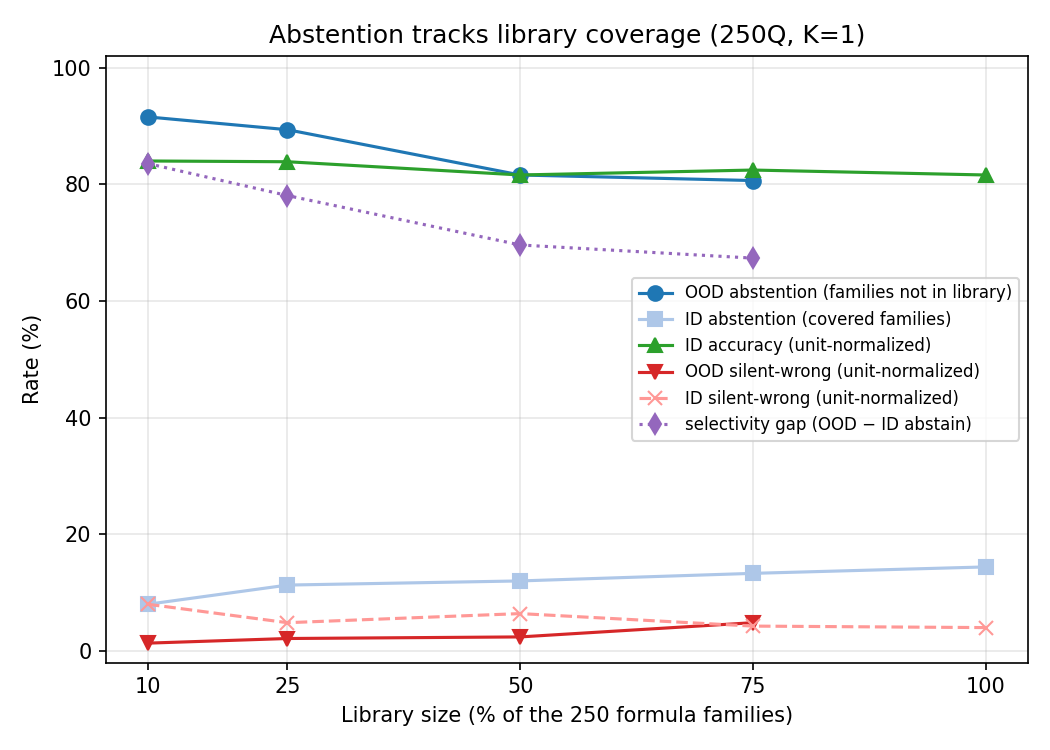
\includegraphics[width=0.94\linewidth]{figures/libsweep_250q.png}
\caption{Library-size sweep ($K{=}1$, nested pristine subset libraries).
Abstention tracks coverage: the out-of-library vs.\ in-library abstention gap holds at every size, while in-library accuracy is flat as the library grows $10\times$.}
\label{fig:v2libsweep}
\end{figure}
But this is a trade-off, not a third victory: on the same out-of-library questions R-PAL answers far more, and does so at \oodRPALcorrOOD{} correct, drawing on parametric knowledge.
VerifiQuant is not more accurate out of library---its own out-of-library selective accuracy is lower (\oodVQselOOD{} vs.\ \oodRPALselOOD{})---and its abstention does not reduce silent-wrong risk there.
What it provides is a \emph{verified/unverified boundary}: it emits a number only when a contract applies, whereas execution and prompting emit confident numbers they cannot vouch for.

\section{Boundary and Failure Analysis}\label{sec:v2boundary}
We consolidate the conditions, failures, and cost of the guarantee here rather than scattering caveats.

\emph{Where the claim holds.}
The empirical claim requires three conditions: the target formula family exists in the library; the contract's specification and invariants are sufficiently correct; and the question is formula-grounded deterministic numerical reasoning.
Where these fail, VerifiQuant provides at most a scope signal, not a correct answer.
The clean-set result is in-library by construction, and out-of-library behavior is exactly the trade-off of RQ3.

\emph{Where failures remain.}
Every residual silent wrong localizes to one of three LLM-mediated \emph{runtime} frontiers, fixed before any run: the \emph{selection} frontier (choosing or force-fitting a near-neighbor contract), the \emph{binding} frontier (extracting or scaling an input wrongly), and the \emph{ambiguity-detection} frontier (failing to recall a declared ambiguity the contract already carries).
No residual across ${\sim}300$ evaluated questions falls outside these three, which tells a deployment team where the next improvement lies rather than reporting an opaque aggregate.
A separate class of \emph{build-time specification defects}---a contract that omits an ambiguity or encodes a wrong invariant---is caught by the contract audits of \S\ref{sec:v2method}, not at runtime.
The ambiguity-detection frontier is already partly mechanized: a deterministic trigger pre-pass fires a declared ambiguity when its convention phrase appears verbatim, moving that hint-recall component out of LLM judgment and cutting SWR further at a small, explicit coverage cost.

\emph{Recoverability.}
Clarification recovers part of the abstained mass.
Truncating the same run (Table~\ref{tab:v2kabl}), VerifiQuant answers autonomously at $81.2\%$ accuracy ($K{=}1$) and, with the intent-aware oracle, at \vqAccAll{} ($K{=}3$), converting abstentions into correct answers while keeping SWR approximately flat.

\begin{table}[t]
\caption{Oracle-budget truncation of the same $K{=}3$ run.
$K{=}1$ is autonomous; clarification converts abstentions into correct answers at an interaction cost, and the oracle sees the intent specification but never the numeric answer.}
\label{tab:v2kabl}
\small
\begin{tabular}{@{}lrrrr@{}}
\toprule
Budget & Acc & SWR & Coverage & Sel.\,Acc \\
\midrule
$K{=}1$ (autonomous) & 81.2\% & 2.8\% & 84.0\% & 96.7\% \\
$K{=}2$ & 92.4\% & 3.6\% & 96.0\% & 96.2\% \\
$K{=}3$ & \vqAccAll{} & \vqSWRAll{} & \vqCovAll{} & \vqSelAccAll{} \\
\bottomrule
\end{tabular}
\end{table}
Because the oracle holds the intent specification, this is an upper bound on clarification benefit, not evidence that an arbitrary user supplies equivalent clarification; we report it as an idealized analysis.

\emph{Remaining limitations.}
VerifiQuant reduces and localizes silent wrongs but does not eliminate them, and residual attribution uses gold answers unavailable in deployment.
The governance advantage is measured on a mechanism-targeted, contract-derived trap set that may favor a contract-gated system; the I\textsubscript{HARD} stratum is small; open-ended intent (M) is unsolved; and results rest on one formula-provenance benchmark and backbone family.
An independently authored, human-labeled messy-query evaluation is the natural external-validity test and is in progress.

\section{Conclusion}
Financial LLM deployment is blocked less by what models get wrong than by what systems cannot govern.
Compiling scope, schema, boundary, and ambiguity checks into an executable funnel makes refusal, clarification, and repair first-class, attributable outcomes.
On well-posed in-library questions a matched retrieval-execution baseline already suffices; the value of executed governance appears on inputs that should not produce a number, where it reduces false numeric acceptance beyond what execution or prompted governance achieve, and on the verified/unverified boundary it maintains when its library ends.
When a gate identifies that the computation cannot be verified, VerifiQuant emits a structured refusal or clarification rather than an unsupported number---which can be preferable in financial deployments that require provenance and reviewable boundaries.
